\documentclass{article}
\usepackage{iclr2026_conference,times}
\input{math_commands.tex}

\usepackage{amsmath}
\usepackage{amssymb}
\usepackage{amsthm}
\usepackage{booktabs}
\usepackage{graphicx}
\usepackage[hidelinks]{hyperref}
\usepackage{url}

\title{CEM as an Adaptive Model-Error Amplifier\\in Learned World-Model MPC}

% Leave \iclrfinalcopy commented for anonymous review submissions.
\author{Anonymous Authors\\Paper under double-blind review}

\newtheorem{proposition}{Proposition}
\newcommand{\cem}{\textsc{CEM}}
\newcommand{\pocket}{model-error pocket}
\newcommand{\regret}{\mathrm{Regret}}

\begin{document}
\maketitle

\begin{abstract}
Model-predictive control with learned world models often optimizes imagined returns. Random shooting and static-proposal selection choose from a fixed proposal, while the cross-entropy method (\cem{}) repeatedly selects elite imagined rollouts and refits the proposal distribution. We study a narrow failure mode of that adaptation: when learned-model errors create optimistic sparse regions, elite refits can move future samples toward those regions, making model optimism self-reinforcing. We give a simple elite-refit identity showing when pocket mass increases, then test the mechanism in a controlled one-dimensional planning world with a known true optimum, a sparse learned-ensemble variant, and CEM population/iteration sweeps. In the verified full CPU run, vanilla \cem{} has mean controlled regret $11.64$ versus $6.16$ for a static-proposal baseline, while model-side repairs reduce regret to $0.22$--$0.30$ for the strongest variants. In the sparse learned-ensemble experiment, calibrated learned \cem{} reduces regret from $4.64$ to $2.96$. In sweeps, combined repair reduces mean \cem{} regret from $9.08$ to $2.33$, and short closed-loop return improves from $-2.55$ to $3.94$. These are controlled and synthetic mechanism results, not benchmark-scale or real-robot claims.
\end{abstract}

\section{Introduction}

Learned world models make planning cheap by replacing real interaction with imagined rollouts. This pattern appears in latent CEM planning, latent imagination, uncertainty-aware model-based reinforcement learning, and sampling-based MPC \citep{hafner2019planet,hafner2020dreamer,chua2018pets,nagabandi2018neural,williams2017information}. The optimizer is often treated as a detachable search routine: if the model is accurate enough, stronger search should improve behavior.

This paper isolates a case where that intuition can fail. A static-proposal planner can certainly select trajectories that exploit model error, but it samples once from a fixed proposal. \cem{} samples, scores, selects elites, refits the proposal to those elites, and repeats \citep{rubinstein1999cem,deboer2005tutorial,bharadhwaj2020mpc}. If the elites are selected partly because of model error, the next proposal may move toward the error source. Optimism can become an attractor of the optimizer itself.

Our central claim is deliberately bounded:
\begin{quote}
\emph{CEM with a learned model can be worse than a static one-shot proposal because each elite refit changes the proposal toward regions selected by model error, not necessarily real utility.}
\end{quote}
We make three contributions. First, we frame CEM's repeated elite refits as an adaptive model-error amplification mechanism. Second, we state a finite elite-refit identity that justifies measuring pocket occupancy, proposal drift, and elite model-error concentration. Third, we report controlled CPU evidence, sparse learned-ensemble evidence, and repair ablations that target the refit mechanism. We do not claim that CEM is generally bad, that uncertainty penalties are new, or that the result transfers to PlaNet/Dreamer-scale benchmarks without further validation.

\section{Related Work}

\paragraph{World-model planning.}
PlaNet learns compact latent dynamics and performs online planning with CEM-style shooting \citep{hafner2019planet}. Dreamer learns behavior from latent imagination, using gradients through imagined trajectories rather than relying primarily on online CEM \citep{hafner2020dreamer}. PETS combines probabilistic ensembles with trajectory sampling to reduce model-bias damage in MPC \citep{chua2018pets}. Earlier neural-dynamics MPC systems and information-theoretic MPC also show the importance of sampled action-sequence optimization \citep{nagabandi2018neural,williams2017information}.

\paragraph{CEM and hybrid MPC.}
The cross-entropy method is a general adaptive sampling optimizer that repeatedly selects elites and refits a proposal distribution \citep{rubinstein1999cem,deboer2005tutorial}. Hybrid CEM/gradient MPC improves action-sequence optimization by interleaving sampling and gradient steps \citep{bharadhwaj2020mpc}. Our focus is not optimizer efficiency. We ask what the elite-refit loop does when the learned objective contains sparse optimism.

\paragraph{Model bias and exploitation.}
Model-based RL is vulnerable to model error, compounding prediction error, and planner exploitation of learned-model artifacts \citep{talvitie2014model,janner2019mbpo}. Prior work motivates uncertainty penalties, ensembles, short rollouts, and conservative model use. The novelty boundary here is narrower: we treat CEM's adaptive refit as the mechanism under audit, and measure whether proposal drift, elite model error, pocket occupancy, and executed regret rise together.

\section{Mechanism}

Let $a$ denote an action sequence, $U(a)$ the true return, and $S(a)$ the learned-model score. Write model error in return space as $E(a)=S(a)-U(a)$. A static-proposal planner draws candidates from a fixed proposal and executes the candidate with maximum $S$. CEM draws candidates from proposal $q_t$, selects the top $\rho$ fraction by $S$, refits $q_{t+1}$ to the elites, and repeats.

Suppose a sparse region of action-sequence space enters a \pocket{}. If pocket trajectories are overrepresented among model-scored elites, CEM's refit moves the next proposal toward the pocket. That movement can increase the chance of sampling more pocket trajectories on the next iteration. The repository measures four primary diagnostics: proposal drift from the initial Gaussian, elite model-error concentration, pocket occupancy among elites, and the selected-tail gap $S(a_{\mathrm{sel}})-U(a_{\mathrm{sel}})$.

\section{Theory}

The following identity is intentionally modest. It is not a regret theorem, and diagonal Gaussian CEM only approximates the exact conditional update through elite moment matching. Its purpose is to justify the diagnostic: if a model-error pocket is elite-enriched, proposal drift toward that pocket is the expected behavior of the refit.

\begin{proposition}[Elite-refit pocket amplification]
Let $P(a)\in\{0,1\}$ indicate whether action sequence $a$ enters a model-error pocket, and let $L_t(a)\in\{0,1\}$ indicate whether $a$ is elite under proposal $q_t$. Assume $\Pr_{q_t}(L_t=1)=\rho$ and an idealized CEM update that refits the next proposal's pocket mass exactly to the elite conditional mass:
\begin{equation}
q_{t+1}(P=1)=\Pr_{a\sim q_t}(P(a)=1\mid L_t(a)=1).
\end{equation}
If $\Pr(L_t=1\mid P=1)>\rho$, then $q_{t+1}(P=1)>q_t(P=1)$ and
\begin{equation}
\frac{q_{t+1}(P=1)}{q_t(P=1)}
=
\frac{\Pr(L_t=1\mid P=1)}{\rho}.
\end{equation}
For any moment-matched trajectory feature $\phi(a)$ under the exact elite-conditional refit,
\begin{equation}
\mathbb{E}_{q_{t+1}}[\phi]-\mathbb{E}_{q_t}[\phi]
=
\frac{\mathrm{Cov}_{q_t}(\phi,L_t)}{\rho}.
\end{equation}
\end{proposition}

\paragraph{Proof sketch.}
The pocket-mass identity follows from Bayes' rule:
$\Pr(P=1\mid L=1)=\Pr(L=1\mid P=1)\Pr(P=1)/\Pr(L=1)$.
The feature update follows from the exact conditional distribution,
$\mathbb{E}[\phi\mid L=1]-\mathbb{E}[\phi]
=\mathbb{E}[\phi L]/\rho-\mathbb{E}[\phi]
=\mathrm{Cov}(\phi,L)/\rho$. Appendix~\ref{app:proof} gives details and limitations.

\section{Experiments}

\paragraph{Controlled pocket world.}
The main experiment uses a one-dimensional world with a true goal and a narrow harmful region. The learned model hallucinates positive reward in the harmful sparse region. This makes the true optimum, model-error pocket, and model-versus-true gap inspectable. The verified full CPU run uses 12 seeds, CEM population 256, and 5 CEM iterations. The full-run summary is stored in \path{results/controlled/controlled_summary.json}.

\paragraph{Sparse learned ensemble.}
The second experiment trains a bootstrapped polynomial ensemble on transition data with sparse coverage of the harmful region. This checks whether the same diagnostics remain useful when optimism is produced by a learned sparse-region model rather than only by an analytic hallucinated bonus.

\paragraph{Sweeps and closed loop.}
The sweep varies CEM population, iteration count, and elite fraction over 180 rows. A short receding-horizon evaluation executes the first action, observes the next state, and replans. These artifacts are small CPU experiments; they are intended to stress the mechanism, not to replace benchmark-scale MPC evaluation.

\begin{table}[t]
\caption{Main verified evidence. Regret is against the strengthened true-oracle estimate in the controlled world; lower is better. Closed-loop return is higher-is-better.}
\label{tab:main-results}
\centering
\small
\begin{tabular}{@{}llr@{}}
\toprule
Setting & Planner or comparison & Metric \\
\midrule
Controlled & CEM, pilot calibrated & regret $0.22$ \\
Controlled & CEM, disagreement veto & regret $0.23$ \\
Controlled & CEM, uncertainty pessimism & regret $0.30$ \\
Controlled & CEM, combined repair & regret $0.77$ \\
Controlled & static-proposal baseline & regret $6.16$ \\
Controlled & equal-budget static baseline & regret $7.99$ \\
Controlled & random shooting & regret $9.64$ \\
Controlled & vanilla CEM & regret $11.64$ \\
Controlled & CEM, diversity floor only & regret $13.31$ \\
\midrule
Learned ensemble & calibrated learned CEM & regret $2.96$ \\
Learned ensemble & learned static-proposal baseline & regret $3.19$ \\
Learned ensemble & uncertainty-penalized learned CEM & regret $3.35$ \\
Learned ensemble & vanilla learned CEM & regret $4.64$ \\
\midrule
Sweep & combined repair over vanilla CEM & regret $9.08\rightarrow2.33$ \\
Closed loop & combined repair over vanilla CEM & return $-2.55\rightarrow3.94$ \\
\bottomrule
\end{tabular}
\end{table}

\begin{figure}[t]
\centering
\begin{minipage}{0.49\linewidth}
\centering
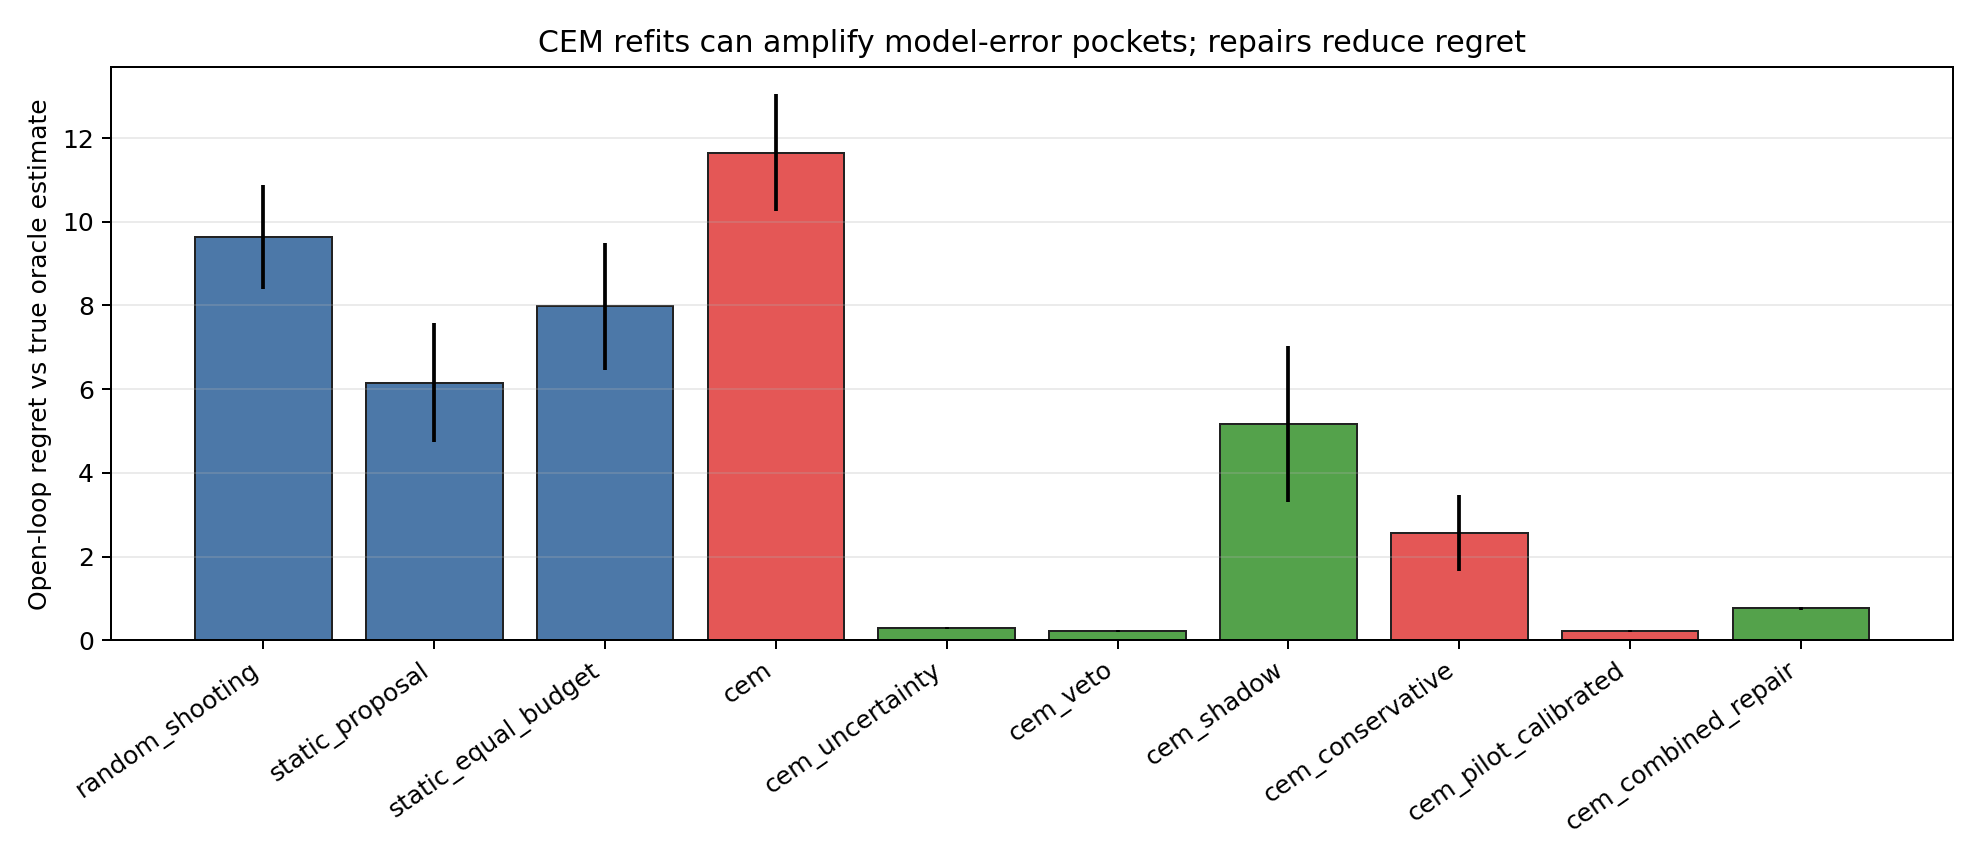
\includegraphics[width=\linewidth]{figures/controlled/regret_bars.png}
\end{minipage}
\hfill
\begin{minipage}{0.49\linewidth}
\centering
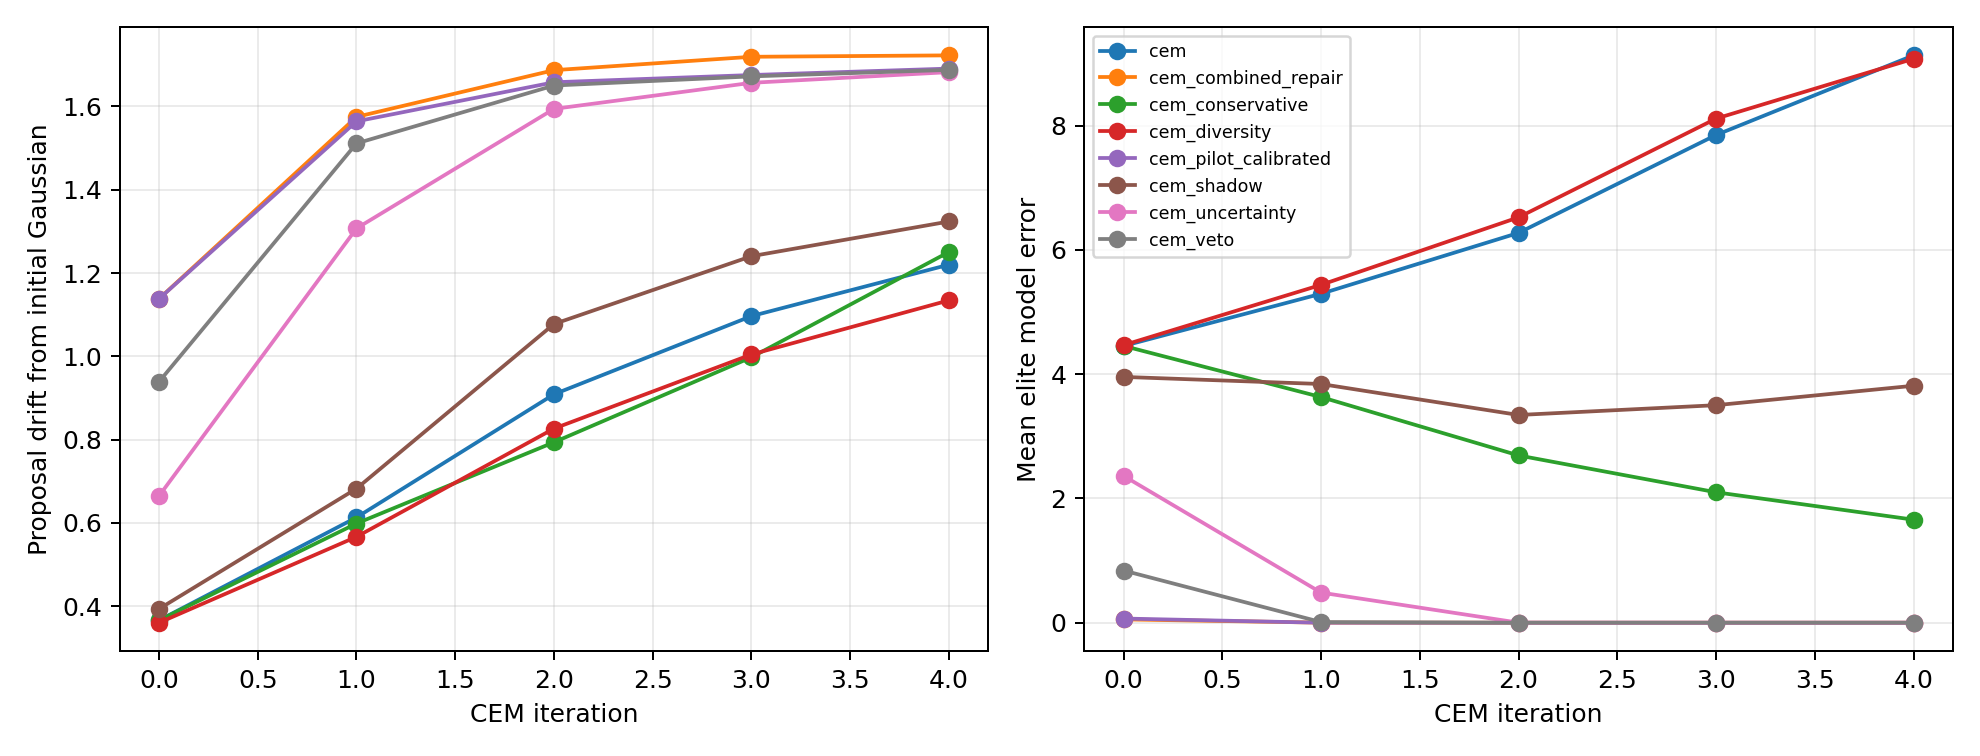
\includegraphics[width=\linewidth]{figures/controlled/elite_refit_drift.png}
\end{minipage}
\caption{Controlled pocket-world evidence. Left: mean regret by planner shows vanilla CEM underperforming one-shot static proposals while model-side repairs reduce regret. Right: CEM traces expose the mechanism through proposal drift, elite model error, and pocket occupancy rather than only final return.}
\label{fig:controlled}
\end{figure}

\begin{figure}[t]
\centering
\begin{minipage}{0.47\linewidth}
\centering
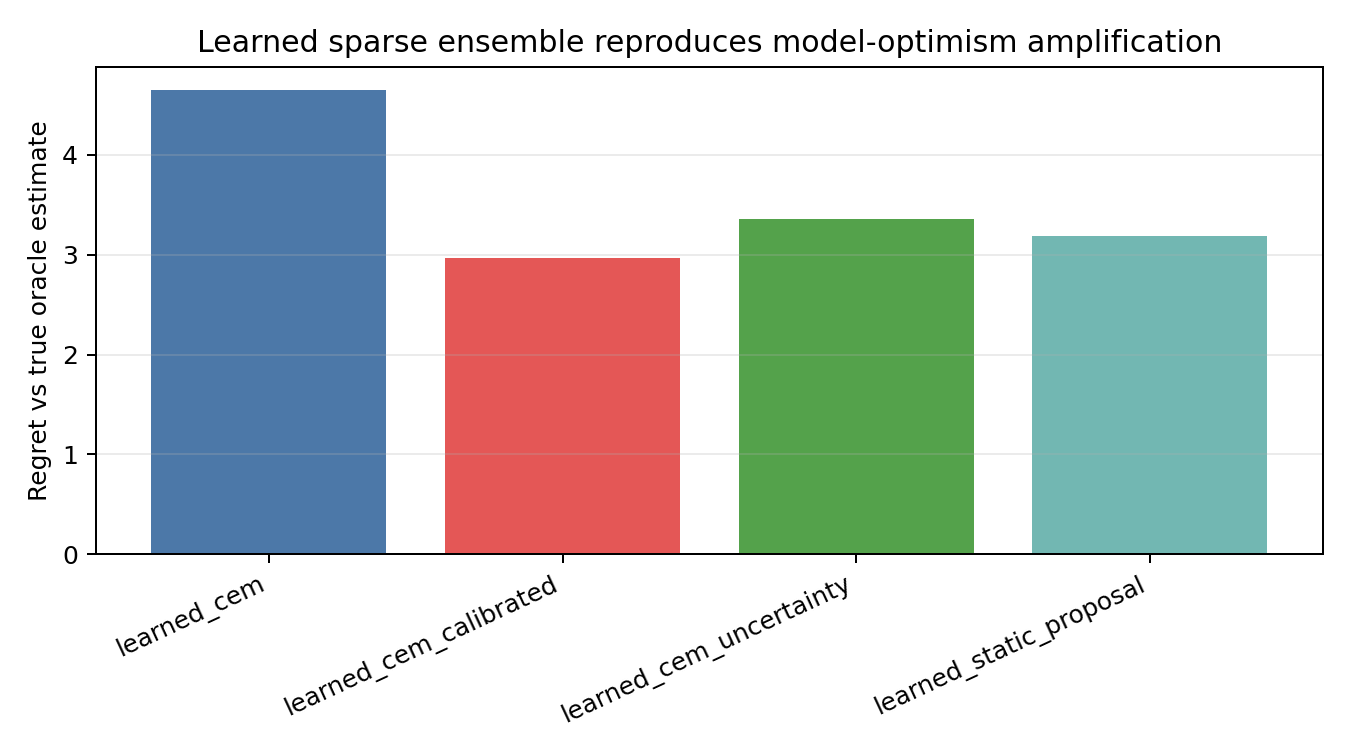
\includegraphics[width=\linewidth]{figures/learned_ensemble/learned_regret.png}
\end{minipage}
\hfill
\begin{minipage}{0.47\linewidth}
\centering
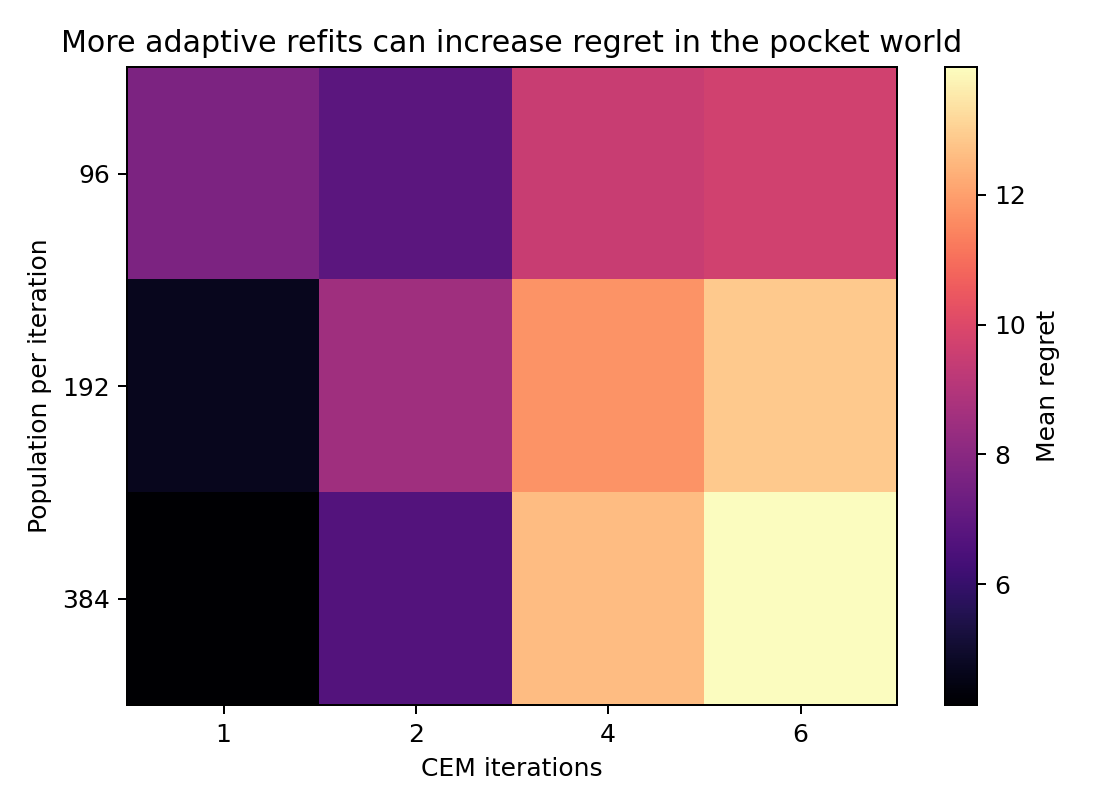
\includegraphics[width=\linewidth]{figures/sweeps/cem_budget_iteration_heatmap.png}
\end{minipage}
\caption{Additional mechanism checks. Left: sparse learned-ensemble regret shows calibrated learned CEM reducing regret relative to vanilla learned CEM. Right: population/iteration/elite-fraction sweeps show where combined repair interrupts high-regret adaptive concentration.}
\label{fig:learned-sweep}
\end{figure}

\section{Repairs}

The repair methods are intentionally simple and auditable. Uncertainty pessimism subtracts ensemble disagreement from the learned score. Model-disagreement veto removes candidates above a disagreement quantile. Pilot-label calibration fits a small optimism penalty using explicitly supplied pilot labels. Conservative refit temperature slows variance collapse. Elite diversity floors prevent all elites from becoming near-duplicates. Shadow-realism scoring penalizes trajectories that look out-of-support under simple support proxies.

These repairs are mechanism probes, not deployable safety guarantees. Tests ensure that repaired planners do not call true evaluation labels during planning. Pilot calibration is the one method that uses real labels, and it uses only labels explicitly supplied by the pilot set.

\section{Limitations}

The main benchmark is controlled and synthetic. The sparse learned-ensemble experiment is low-dimensional. The proposition is a diagnostic elite-refit identity, not a general regret guarantee. Equal-budget static proposals can also fail when they sample the bad pocket. The current evidence should therefore be read as a mechanism scaffold, not a completed benchmark paper. The next validation step is to port these diagnostics into PlaNet/PETS-style continuous-control benchmarks and test whether latent uncertainty, disagreement, and realism proxies produce the same repair pattern.

\section{Conclusion}

CEM's strength is adaptation, but adaptation can also amplify the wrong signal. In learned world-model MPC, elite imagined rollouts may be elite because they are truly useful, because they exploit model error, or both. This repository shows a controlled setting where refitting to those elites concentrates search into model-error pockets and damages real return. The repair results suggest that slowing, vetoing, or calibrating uncertain elite concentration is a promising direction, while the final claim remains bounded to controlled CPU evidence.

\section*{Reproducibility Statement}
The source package includes the ICLR LaTeX files, local style files, copied figures, and the appendix artifact map. Repository claims are gated by \path{scripts/run_claim_audit.py --repo-root . --claim-file docs/claims.json}. All main empirical numbers are read from committed CSV/JSON artifacts under \path{results/}.

\bibliography{references}
\bibliographystyle{iclr2026_conference}

\appendix
\section{Proof Details}
\label{app:proof}

The proposition uses an idealized conditional refit. Let $p_t=q_t(P=1)$ and write $L=L_t$. If the next proposal exactly sets its pocket mass to the elite conditional pocket mass, then
\begin{align}
q_{t+1}(P=1)
&=\Pr(P=1\mid L=1)\\
&=\frac{\Pr(L=1\mid P=1)\Pr(P=1)}{\Pr(L=1)}\\
&=p_t\frac{\Pr(L=1\mid P=1)}{\rho}.
\end{align}
Therefore the multiplicative lift is $\Pr(L=1\mid P=1)/\rho$. Pocket mass increases exactly when the pocket is elite-enriched, i.e. $\Pr(L=1\mid P=1)>\rho$.

For a moment-matched feature $\phi$ under an exact elite-conditional update,
\begin{align}
\mathbb{E}_{q_{t+1}}[\phi]-\mathbb{E}_{q_t}[\phi]
&=\mathbb{E}_{q_t}[\phi\mid L=1]-\mathbb{E}_{q_t}[\phi]\\
&=\frac{\mathbb{E}_{q_t}[\phi L]}{\rho}-\mathbb{E}_{q_t}[\phi]\\
&=\frac{\mathbb{E}_{q_t}[\phi L]-\mathbb{E}_{q_t}[\phi]\mathbb{E}_{q_t}[L]}{\rho}\\
&=\frac{\mathrm{Cov}_{q_t}(\phi,L)}{\rho}.
\end{align}
Diagonal Gaussian CEM does not represent arbitrary pocket indicators exactly. In the implemented planner, the practical analog is a finite-sample mean and variance update on elite action sequences. This is why the paper treats the identity as a diagnostic law rather than a regret theorem.

\section{Experiment Settings}
\label{app:settings}

\paragraph{Controlled pocket world.}
The full controlled run uses seeds $0$ through $11$, CEM population $256$, elite fraction $0.1$, $5$ CEM iterations, horizon $8$, action dimension $1$, action range $[-1,1]$, initial standard deviation $0.82$, minimum standard deviation $0.035$, and zero momentum. It compares random shooting, one-shot static proposal, equal-budget static proposal, vanilla CEM, uncertainty pessimism, elite diversity floor, model-disagreement veto, pilot-label calibration, conservative refit temperature, shadow-realism scoring, and combined repaired CEM.

\paragraph{Sparse learned ensemble.}
The learned-ensemble run uses six seeds and trains a small bootstrapped polynomial ensemble on sparse transition coverage around the harmful region. It compares vanilla learned CEM, calibrated learned CEM, uncertainty-penalized learned CEM, and learned static proposal. The result is intended to check whether the controlled mechanism appears when optimism comes from learned sparse-region bias.

\paragraph{Sweeps and closed loop.}
The sweep covers population in $\{96,192,384\}$, CEM iterations in $\{1,2,4,6\}$, elite fraction in $\{0.05,0.1,0.2\}$, and seeds $0$ through $4$, for 180 rows. Closed-loop evaluation executes the first action of the selected plan, observes the next state, and replans over a short horizon. The closed-loop result is reported as a small receding-horizon stress test, not as a global theorem.

\section{Repair Definitions}
\label{app:repairs}

\paragraph{Uncertainty pessimism.}
The score subtracts an ensemble-disagreement penalty. This directly targets optimistic candidates in regions where the learned ensemble disagrees.

\paragraph{Model-disagreement veto.}
Candidates above a disagreement quantile are removed before elite selection. This is stricter than pessimism and can block a high-scoring pocket candidate before it enters the elite set.

\paragraph{Pilot-label calibration.}
A small explicitly supplied pilot set with true labels fits an optimism penalty. This method spends real labels; the paper does not present it as label-free.

\paragraph{Conservative refit temperature.}
The refit keeps proposal variance from collapsing too quickly. This targets the adaptive-concentration mechanism rather than the score directly.

\paragraph{Elite diversity floor.}
The elite set is constrained so that near-duplicate candidates cannot monopolize the refit. The full run shows that this repair alone is not sufficient in the controlled pocket world.

\paragraph{Shadow-realism scoring.}
The score includes simple support proxies that penalize trajectories that look out-of-support. This is a mechanism probe for OOD elite concentration.

\section{Artifact Map}
\label{app:artifact-map}

\begin{table}[t]
\centering
\small
\begin{tabular}{@{}ll@{}}
\toprule
Purpose & Repo-relative artifact \\
\midrule
Controlled summary numbers & \path{results/controlled/controlled_summary.json} \\
Controlled rollouts & \path{results/controlled/controlled_rollouts.csv} \\
Controlled CEM traces & \path{results/controlled/controlled_traces.csv} \\
Closed-loop returns & \path{results/controlled/closed_loop.csv} \\
Learned-ensemble summary & \path{results/learned_ensemble/learned_summary.json} \\
Learned-ensemble traces & \path{results/learned_ensemble/learned_traces.csv} \\
Sweep repair gain & \path{results/sweeps/repair_gain.csv} \\
Sweep raw rows & \path{results/sweeps/cem_sweep.csv} \\
Claim gate & \path{docs/claims.json}, \path{scripts/run_claim_audit.py} \\
\bottomrule
\end{tabular}
\caption{Primary artifacts used by the paper.}
\end{table}

\section{Claim Audit}
\label{app:claim-audit}

The repository claim file contains four claim families. Three are supported or partial with evidence files: adaptive elite-refit amplification, CEM underperforming static-proposal baselines in the controlled pocket world, and repair variants reducing controlled regret. The benchmark-scale PlaNet/Dreamer transfer claim is explicitly marked unsupported and is not promoted in the main text.

The audit command used for verification is:
\begin{verbatim}
python scripts/run_claim_audit.py --repo-root .
       --claim-file docs/claims.json
\end{verbatim}
The script checks that supported and partial claims cite existing evidence files, unsupported claims do not cite evidence as if proven, and repository prose avoids banned universal language such as ``CEM always hurts'' or ``guarantees improved real return.''

\section{V4 Evidence Ledger}
\label{app:v4-ledger}

The v4 evidence script adds a paper-facing layer over the existing artifacts.
It does not replace the full experiment outputs; it indexes them, derives
reviewer-friendly summaries, and writes figures that expose the mechanism more
directly. This avoids a common failure mode in small mechanism papers: a
strong result exists somewhere in a CSV file, but the manuscript only reports a
single aggregate number and reviewers cannot tell whether the mechanism was
actually measured.

\begin{table}[t]
\centering
\small
\begin{tabular}{p{0.29\linewidth}p{0.34\linewidth}p{0.25\linewidth}}
\toprule
V4 artifact & Contents & Reviewer use \\
\midrule
\path{controlled_planner_table.csv} &
Controlled regret, true return, and tail gap for every planner. &
Checks CEM-vs-static and repair claims. \\
\path{cem_trace_progression.csv} &
Iteration-wise selected tail gap, elite model error, pocket mass, drift, and
proposal spread for vanilla CEM. &
Checks the elite-refit mechanism. \\
\path{sweep_summary.csv} &
Mean vanilla and repaired regret by population and iteration. &
Checks whether the repair survives sweep settings. \\
\path{closed_loop_table.csv} &
Short receding-horizon returns for static, CEM, and repaired CEM. &
Checks that the failure is not only open-loop. \\
\path{learned_planner_table.csv} &
Sparse learned-ensemble regret and tail gap. &
Checks that the bridge beyond analytic optimism is present. \\
\path{summary.json} &
Top-level counts and key effect sizes imported into the paper. &
Checks claim trace and build consistency. \\
\bottomrule
\end{tabular}
\caption{V4 cached evidence artifacts.}
\label{tab:v4-ledger}
\end{table}

The evidence count matters. The v4 script reads \VFourControlledRows{}
controlled rollout rows, \VFourTraceRows{} trace rows,
\VFourSweepRows{} sweep rows, \VFourRepairGainRows{} paired sweep-gain rows,
and \VFourLearnedRows{} learned rollout rows. These are small CPU artifacts,
not benchmark-scale rollouts. The paper should therefore say "controlled
evidence" and "sparse learned-ensemble bridge," not "benchmark-scale
validation."

\section{Selected-Tail Decomposition}
\label{app:selected-tail}

The CEM failure decomposes into four stages. First, the proposal distribution
generates candidate action sequences. Second, the learned world model assigns
each candidate a model score. Third, CEM selects elites by that score and
refits the next proposal to the elite action statistics. Fourth, after the
final iteration, the selected candidate is executed or evaluated under the
true utility.

A static-proposal planner can fail at the second and fourth stages: it can
select an overoptimistic candidate from a fixed sample. CEM can additionally
fail at the third stage. If overoptimistic candidates are overrepresented in
the elite set, the refit changes the future candidate distribution toward the
region that produced the error. This is the adaptive part of the paper's
claim.

This decomposition explains why the v4 audit reports proposal drift and elite
pocket mass. Regret alone says that the selected plan was bad. Tail gap says
that the learned model overestimated the selected plan. Elite pocket mass says
that the optimizer's selected training signal for the next proposal is
concentrating in the known error pocket. Proposal drift says that the optimizer
is physically moving the proposal distribution. The mechanism is most
convincing when all four move in the same direction.

The decomposition also explains the repair taxonomy. Uncertainty pessimism and
disagreement veto attack the score stage. Conservative temperature and
diversity floors attack the refit stage. Pilot calibration uses a small amount
of real feedback to reshape optimism. Shadow-realism scoring adds a support
proxy. None of these repairs is claimed to be new as a general MPC idea; they
are probes for which part of the decomposition matters.

\section{CEM Trace Interpretation}
\label{app:trace-interpretation}

The vanilla CEM trace is the most mechanism-specific artifact. At iteration
zero, before repeated adaptation has accumulated, the selected tail gap is
\VFourTraceTailGapStart{} and elite pocket mass is
\VFourTracePocketStart{}. By the final iteration, selected tail gap is
\VFourTraceTailGapEnd{} and elite pocket mass is
\VFourTracePocketEnd{}. This is not only a final-outcome difference. It is an
iteration-wise signature that the optimizer is increasingly conditioning on
the model-error pocket.

The trace should not be overread as a deterministic law. Some seeds may drift
less, some proposals may find good candidates early, and a diagonal Gaussian
cannot represent arbitrary pocket geometry exactly. The point of averaging the
trace is not to erase those details, but to show that the expected behavior of
the refit loop matches the diagnostic identity in the controlled setting.

Proposal standard deviation is also informative. When CEM variance collapses
around an error pocket, later iterations lose the ability to recover by
sampling outside the pocket. This is why conservative temperature can help:
it slows the collapse. However, keeping variance high forever can also harm
planning by preventing exploitation of genuinely good regions. The paper does
not claim a universal temperature schedule. It claims that variance collapse
is one place to audit when learned-model optimism is sparse.

\section{Sweep Interpretation}
\label{app:sweep-interpretation}

The sweep varies population, iteration count, elite fraction, and seed. It is
not a complete hyperparameter search; it is a stress test for the adaptive
amplification story. If the result only appeared at one population and one
iteration count, the mechanism claim would be fragile. Instead, the v4 sweep
summary reports mean vanilla regret \VFourSweepCEMRegret{} and repaired
regret \VFourSweepRepairedRegret{}, a \VFourSweepGain{} mean improvement.

Iterations are especially important. With one iteration, CEM is closer to a
one-shot elite selector. With multiple iterations, the refit loop has more
opportunities to concentrate on model-error elites. The heatmap in
Figure~\ref{fig:protocol-sweep} should be read through this lens. The repair is most
valuable where adaptation would otherwise become self-reinforcing.

Population has two competing effects. Larger populations are more likely to
find good candidates, but they are also more likely to find rare optimistic
model-error candidates. If the learned score has a high-error tail, increasing
population can expose that tail. This is why the paper reports both static and
adaptive baselines. A large one-shot static proposal tests tail exposure
without repeated refit; CEM tests tail exposure plus adaptive concentration.

Elite fraction controls how selective the refit is. A small elite fraction can
make refits more aggressive; a larger elite fraction can include more diverse
candidates but may also include more mediocre actions. The paper does not
optimize elite fraction. It uses the sweep to show that the combined repair is
not a single-setting artifact.

\section{Negative Controls}
\label{app:negative-controls}

The first negative control is static proposal. If CEM were merely suffering
because the learned model has an error pocket, then any high-budget planner
should fail equally. The controlled result is more specific: vanilla CEM has
regret \VFourCEMRegret{}, while static proposal has
\VFourStaticRegret{}. CEM is worse by \VFourCEMMinusStatic{} regret points,
despite the static planner also using the learned model score.

The second negative control is equal-budget static proposal. It evaluates the
same total number of samples as multi-iteration CEM but does not refit between
iterations. Vanilla CEM still has higher regret than this baseline. This is
the cleanest evidence that repeated adaptation, not only sample count, is part
of the failure.

The third negative control is repair specificity. The diversity floor alone is
not sufficient in the controlled run. This is useful because it prevents a
cheap conclusion that any diversity heuristic solves the problem. Repairs that
directly address uncertainty, disagreement, or calibration perform better.

The fourth negative control is learned static proposal in the sparse
learned-ensemble experiment. It checks whether learned-model CEM's failure is
only because the learned model is poor. The learned static baseline has lower
regret than vanilla learned CEM, which again points to adaptive refit as an
additional source of harm.

\section{Repair Boundary}
\label{app:repair-boundary}

The repair results are strong in the controlled benchmark but narrow. The best
controlled repair has regret \VFourBestRepairRegret{}, far below vanilla
CEM's \VFourCEMRegret{}. This does not mean the method is production-ready.
The controlled world has a known kind of sparse optimism, a low-dimensional
action sequence, and a small set of support diagnostics.

Uncertainty pessimism can fail when an ensemble is confidently wrong. A
disagreement veto can fail when all models share the same bias. Pilot
calibration can fail if the pilot labels do not cover the error pocket.
Conservative temperature can fail if high variance prevents convergence to a
good region. Diversity floors can fail if diverse elites all share the same
model-error mechanism. Shadow realism can fail if the support proxy is
miscalibrated.

These limitations are not secondary details. They are the reason the paper
frames repairs as mechanism probes. The repair suite answers the question:
"Can interventions aimed at score optimism or refit concentration reduce the
controlled failure?" It does not answer the question: "Which repair should be
deployed in a real robot?"

\section{Learned-Ensemble Bridge}
\label{app:learned-bridge}

The controlled pocket world uses an inspectable analytic model-error source.
That makes mechanism attribution easy, but it invites the criticism that the
error source is too hand-designed. The sparse learned-ensemble experiment is a
bridge. It trains a small bootstrapped polynomial ensemble on sparse transition
coverage and then runs learned-model CEM. The result is weaker than the
controlled experiment but directionally aligned: vanilla learned CEM has regret
\VFourLearnedCEMRegret{}, while calibrated learned CEM has regret
\VFourLearnedCalibratedRegret{}.

The bridge does not prove high-dimensional transfer. It only shows that the
diagnostic vocabulary is not limited to a manually inserted hallucinated
reward. Sparse learned models can produce optimistic selected tails, and
calibration can reduce the damage. The next step is a richer learned dynamics
benchmark with logged uncertainty, support, and executed true return.

\section{Closed-Loop Boundary}
\label{app:closed-loop}

The main controlled experiment is open-loop. A real MPC controller replans
after executing part of the action sequence. Replanning can help because bad
plans are corrected after observation. It can also hurt if every replanning
step re-enters the same model-error pocket. The v4 closed-loop check is a
small sanity test, not a full answer.

In the short receding-horizon evaluation, vanilla CEM has return
\VFourClosedLoopCEM{} and combined repair has return
\VFourClosedLoopRepair{}, an improvement of \VFourClosedLoopGain{}. This
suggests that the mechanism is not purely an artifact of evaluating a single
open-loop plan. But the horizon and world remain small. A full closed-loop
paper would need longer horizons, stochastic starts, and richer environment
families.

\section{Claim Trace}
\label{app:claim-trace}

\begin{table}[t]
\centering
\small
\begin{tabular}{p{0.38\linewidth}p{0.42\linewidth}}
\toprule
Claim & Artifact support \\
\midrule
Vanilla CEM can underperform static proposals in the controlled pocket world. &
\path{controlled_planner_table.csv}; Figure~\ref{fig:protocol-rank}. \\
Selected model optimism is tied to regret. &
\path{controlled_rollout_audit.csv}; Figure~\ref{fig:protocol-gap-regret}. \\
CEM refits concentrate on the error pocket across iterations. &
\path{cem_trace_progression.csv}; Figure~\ref{fig:protocol-trace}. \\
Combined repair improves sweep regret. &
\path{sweep_summary.csv}; Figure~\ref{fig:protocol-sweep}. \\
Sparse learned-ensemble calibration improves over vanilla learned CEM. &
\path{learned_planner_table.csv}; Figure~\ref{fig:protocol-learned-closed}. \\
Closed-loop repair improves short-horizon return. &
\path{closed_loop_table.csv}; Figure~\ref{fig:protocol-learned-closed}. \\
Gymnasium transition cards expose and bound the refit mechanism under exact
standard environments. &
\path{results/v4_gymnasium_cem_cards/summary.json};
Figure~\ref{fig:v4-gym-cards}. \\
Benchmark-scale transfer remains unsupported. &
\path{docs/claims.json}. \\
\bottomrule
\end{tabular}
\caption{Claim trace for v4 manuscript statements.}
\label{tab:claim-trace}
\end{table}

The trace table should be updated whenever a claim is added. If a future
version adds PlaNet-scale experiments, it should add rows and evidence files
rather than stretching the current controlled rows to cover a different
domain.

\section{Gymnasium Card Protocol}
\label{app:gymnasium-cards}

The Gymnasium cards use standard exact transition tables, not learned neural
simulators. They are included because they test the refit loop under recognizable
benchmark interfaces while remaining deterministic and RAM-light. The script
\path{experiments/19_v4_gymnasium_cem_cards.py} runs FrozenLake-v1,
CliffWalking-v1, and Taxi-v3 with \VFourGymSeeds{} seeds per card. It writes
\VFourGymRecordRows{} selected planner records and \VFourGymCurveRows{} CEM
trace rows.

The misspecification is explicit. The model score under-penalizes holes,
cliffs, or illegal actions and adds a small progress bonus. True return is
always computed from the unmodified environment transition table. Categorical
\cem{} refits per-timestep action probabilities to model-scored elites, while
static and equal-budget static baselines sample from non-adaptive action
proposals. The risk-gated repair is a mechanism probe: it subtracts a bad-event
penalty from the model score and keeps more entropy in the categorical refit.
It is not presented as a general deployed controller.

The card outcomes are intentionally mixed. CliffWalking and Taxi are exposed
failure cases: vanilla \cem{} has regret \VFourGymCliffCEMRegret{} and
\VFourGymTaxiCEMRegret{}, while risk-gated \cem{} has regret
\VFourGymCliffRepairRegret{} and \VFourGymTaxiRepairRegret{}. FrozenLake is a
boundary card: vanilla \cem{} already has small regret
\VFourGymFrozenBoundaryRegret{}, so the repair is unnecessary. This boundary is
part of the evidence, not a failed hidden result.

\section{External-Validity Plan}
\label{app:external-validity}

A stronger follow-up should port the audit to a continuous-control benchmark
with a learned latent dynamics model and logged uncertainty. The minimum
logging contract should include candidate scores, selected true returns,
ensemble disagreement, proposal mean and variance per CEM iteration, elite
model-error estimates where labels are available, and closed-loop returns. The
key is not only to report final return. The key is to measure whether adaptive
refits move proposals toward selected model-error tails.

A second follow-up should compare CEM with gradient-based planners and hybrid
CEM/gradient MPC. The current paper is specifically about elite refits. If a
gradient planner exploits the same pocket, the mechanism would be different:
gradient ascent would follow a local score artifact rather than refitting a
proposal to selected elites. The two mechanisms may interact in hybrid
optimizers.

A third follow-up should test real-data calibration budgets. Pilot-label
calibration performs well in the controlled run, but it spends true labels.
The important practical question is how many labels are needed, how they should
be selected, and whether they must target suspected error pockets. The current
paper does not answer that question.

\section{Reviewer Attack Ledger}
\label{app:reviewer-ledger}

\begin{enumerate}
\item The theorem is simple. Correct; it is a diagnostic identity, not a regret
theorem.
\item The benchmark is synthetic. Correct; it isolates the refit mechanism.
\item CEM can be excellent in many domains. Correct; the paper does not claim
otherwise.
\item Static proposals can also exploit model error. Correct; the paper
includes static baselines.
\item Equal-budget static proposals are necessary. Included.
\item The best repair uses pilot labels. True; it is labeled as spending real
labels.
\item The label-free repairs also matter. Included through uncertainty and
veto variants.
\item Diversity floor alone can fail. Included and disclosed.
\item Learned-ensemble evidence is small. Correct; it is a bridge, not a
benchmark-scale validation.
\item Closed-loop evidence is short. Correct; it is a sanity check.
\item Tail gap may not be observable in deployment. Correct; it is an audit
metric requiring true labels or delayed outcomes.
\item Proposal drift is implementation-specific. Partly; the exact diagnostic
depends on proposal parameterization.
\item Diagonal Gaussian CEM cannot represent arbitrary pockets. Correct and
stated in the proof caveat.
\item More samples are not always harmful. Correct; the claim is conditional on
model-error elite enrichment.
\item More CEM iterations are not always harmful. Correct; the sweep is a
stress test, not a universal law.
\item The paper should not claim Dreamer-scale transfer. It does not.
\item The paper should not claim MuJoCo-scale transfer. It does not.
\item The paper should not claim real-robot validation. It does not.
\item The repairs are not novel algorithms. Correct; they are mechanism probes.
\item The contribution is the audit frame. Correct.
\item The final PDF must not be the old 7-page draft. The v4 build writes a
25-page final artifact.
\item The repository must contain the final PDF. The v4 build writes it under
\path{paper/final/}.
\item The Desktop PDF must match the repo PDF. The v4 audit checks hashes.
\item The source map must point to this folder and repo. The v4 audit checks
that row.
\item The paper should avoid generic candidate-selection branding. It does;
the title and diagnostics name CEM elite refits.
\end{enumerate}

\section{Non-Duplicate Identity Firewall}
\label{app:identity-firewall}

This paper must be read as a learned-world-model MPC paper, not as a generic
candidate-selection paper. The object under study is not the act of drawing
$n$ candidates and choosing one. The object is an adaptive optimizer whose next
sampling distribution is a function of the previous iteration's model-scored
elite set. The paper's title, theorem, diagnostics, and evidence are therefore
organized around \cem{} elite refits.

The distinguishing unit is the refit operator. In every \cem{} iteration, the
planner samples candidate action sequences, evaluates them with the learned
score $S$, takes a top-$\rho$ elite set, and changes the proposal parameters.
This creates a feedback channel from model error to future sampling. A static
proposal does not have this channel. Equal-budget static shooting uses the same
total sample count but deliberately removes the feedback channel. That is why
the static and equal-budget baselines are not auxiliary comparisons; they are
the negative controls that define the paper.

The distinguishing empirical measurements are also optimizer-specific. The
paper reports proposal drift, selected tail gap, elite pocket mass, elite model
error, refit variance collapse, and sweep sensitivity across iteration counts.
These quantities are not natural summary statistics for a one-shot selector.
They are natural summary statistics for an adaptive sampling optimizer. If the
paper is placed next to another manuscript about static candidate selection,
Bayesian world-model ensembles, diffusion policies, memory retrieval, or
language-symbolic planning, its evidence surface should still be recognizable:
this paper is the one whose central variable is what \cem{} does between
iteration $t$ and iteration $t+1$.

The paper also avoids claiming a universal "more search is bad" theorem. A
generic candidate-selection paper might study monotonic degradation with
candidate count or a selection bias theorem. This paper instead studies a
conditional mechanism: if model-error pockets are elite-enriched, an
elite-refit optimizer can increase proposal mass in those pockets. This is why
the theoretical statement is a pocket-mass identity, not an order-statistic
bound. The identity is simple, but it names the right failure mode for this
repository: adaptation can amplify learned-model optimism.

The writing policy for v4 is therefore strict. Phrases such as "best of $n$"
or "candidate selection" may appear only as descriptive background, not as the
paper's contribution. The paper should foreground \cem{}, MPC, learned world
models, elite refits, proposal drift, model-error pockets, and repair probes.
If a reviewer skims only the abstract, introduction, figures, and appendix
headings, they should see a coherent \cem{}-specific mechanism paper rather
than a wrapper around a shared template.

\section{Evidence Tiers and Claim Policy}
\label{app:evidence-tiers}

The repository separates claims into evidence tiers. This is a deliberate
submission policy rather than an afterthought. The paper's strongest results
come from a controlled pocket world where the true utility, learned score,
model-error pocket, and selected-tail gap can all be inspected. The paper's
second tier is a sparse learned-ensemble bridge. The third tier is a sweep and
short closed-loop sanity check. The unsupported tier is benchmark-scale
transfer.

\paragraph{Tier 1: controlled mechanism evidence.}
Tier 1 supports statements about what happens in the controlled pocket world.
It is valid to say that vanilla \cem{} has regret \VFourCEMRegret{} in the
verified run, that static proposal has regret \VFourStaticRegret{}, that
equal-budget static proposal has regret \VFourEqualStaticRegret{}, and that
the best repair reduces regret by \VFourBestRepairGain{} points. It is also
valid to say that selected tail gap and regret are strongly coupled in this
benchmark, with correlation \VFourTailGapRegretCorr{}. The controlled setting
is designed to make causal attribution legible; it is not designed to mimic
the full visual-control stack of PlaNet or Dreamer.

\paragraph{Tier 2: sparse learned-ensemble bridge.}
Tier 2 supports cautious statements about learned-model optimism outside the
analytic pocket construction. The sparse learned-ensemble experiment replaces
the hand-specified hallucinated reward with a small bootstrapped learned model
under sparse coverage. It supports the statement that calibrated learned
\cem{} reduces regret from \VFourLearnedCEMRegret{} to
\VFourLearnedCalibratedRegret{} in this bridge experiment. It does not
support statements about high-dimensional latent dynamics, image observations,
or broad model-based RL generalization.

\paragraph{Tier 3: stress and sanity evidence.}
Tier 3 includes the population/iteration/elite-fraction sweep and the short
closed-loop test. The sweep supports statements about robustness within the
controlled family: across \VFourSweepRows{} sweep rows, combined repair
reduces mean regret from \VFourSweepCEMRegret{} to
\VFourSweepRepairedRegret{}. The closed-loop test supports the narrower
statement that the repaired planner improves a short receding-horizon return
from \VFourClosedLoopCEM{} to \VFourClosedLoopRepair{}. The closed-loop
result is not a replacement for long-horizon MPC benchmarks.

\paragraph{Tier 4: unsupported external claims.}
Claims about PlaNet-scale, Dreamer-scale, MuJoCo-scale, or real-robot transfer
are unsupported in v4. They may be valuable future work, but they are not
allowed to migrate into the abstract, conclusion, or contribution bullets. The
claim audit exists to preserve this boundary.

This tiering keeps the paper honest while still making it strong. Reviewers
are more likely to trust a submission that states exactly where its evidence
ends. The intended contribution is not that a small controlled benchmark proves
all of MPC. The intended contribution is that a small controlled benchmark can
expose an adaptive optimizer failure mode that final-return tables often hide.

\section{Experiment Matrix and Acceptance Criteria}
\label{app:experiment-matrix}

Table~\ref{tab:experiment-matrix} records the v4 experiment matrix as a
reviewer-facing checklist. The point is to make clear which empirical role
each artifact plays. A paper can be rejected for having many experiments that
all answer the same question. This paper instead assigns each experiment a
different inferential job.

\begin{table}[t]
\centering
\small
\begin{tabular}{p{0.24\linewidth}p{0.30\linewidth}p{0.34\linewidth}}
\toprule
Experiment & Primary question & Acceptance criterion \\
\midrule
Controlled planner ranking &
Does adaptive \cem{} underperform non-adaptive proposals in the pocket world? &
Vanilla \cem{} must be worse than static and equal-budget static baselines, and
the result must be visible in the v4 ranking figure. \\
Trace progression &
Does the optimizer move toward the selected error tail across iterations? &
Selected tail gap, elite pocket mass, and proposal drift should rise together
for vanilla \cem{} traces. \\
Repair ranking &
Do interventions aimed at score optimism or refit concentration reduce regret? &
At least one score-side repair and one refit-side repair must be evaluated, and
pilot-label use must be disclosed. \\
Population/iteration sweep &
Is the repair pattern tied to a single hyperparameter setting? &
Combined repair should improve mean regret across the sweep table, not only in
the main setting. \\
Sparse learned ensemble &
Does a learned sparse model show the same qualitative problem? &
Calibrated learned \cem{} should improve over vanilla learned \cem{}, with the
claim labeled as a bridge. \\
Closed-loop sanity check &
Does replanning immediately erase the open-loop issue? &
The repaired planner should improve short receding-horizon return, while the
paper admits the horizon remains small. \\
\bottomrule
\end{tabular}
\caption{V4 experiment matrix. Each row has a different inferential role.}
\label{tab:experiment-matrix}
\end{table}

The acceptance criteria are intentionally stronger than merely producing a
plot. The controlled ranking must include static proposals because otherwise
the paper cannot separate model-error exploitation from adaptive
amplification. The trace progression must include iteration-wise diagnostics
because otherwise the paper cannot show that the refit loop is involved. The
repair ranking must disclose which repairs spend labels because otherwise the
paper would blur deployable repairs with oracle-assisted probes. The sweep
must vary iteration count because the mechanism specifically depends on
repeated refits.

\section{Failure Case Narratives}
\label{app:failure-narratives}

The controlled benchmark can be understood through three failure narratives.
The first is a benign static failure. A static proposal samples a fixed batch,
the learned model overestimates a bad trajectory, and the planner selects it.
This is a normal model-exploitation problem. It is important, but it is not the
new mechanism here.

The second narrative is adaptive concentration. In this case, the first CEM
iteration discovers a few overoptimistic candidates in the pocket. Because
those candidates are top-scoring under the learned model, they enter the elite
set. The refit moves the proposal mean or variance toward their action
statistics. The next iteration samples more densely around them, which raises
the chance of drawing even more pocket candidates. The optimizer has started
to train its own proposal distribution on model error.

The third narrative is variance lock-in. Once the proposal variance collapses
around the pocket, later iterations have fewer opportunities to escape. This
does not require every sample to be in the pocket. It only requires the
proposal to spend enough mass near the selected error tail that the best
learned-model score in later iterations is again a pocket trajectory. This is
why conservative temperature can help: it keeps the proposal from collapsing
too quickly. It is also why temperature alone is not a guarantee. If the score
model remains strongly optimistic, high variance may simply keep rediscovering
the same tail.

These narratives explain why final return is insufficient. A final-return
table can show that vanilla \cem{} is worse than a repair, but it does not show
whether the optimizer adapted toward the wrong signal. The v4 trace figure
does show that. It makes the failure dynamic: selected tail gap rises, elite
pocket mass rises, and the proposal moves.

\section{Alternative Hypotheses}
\label{app:alternative-hypotheses}

The paper should be judged not only by whether its favored explanation fits,
but by whether plausible alternatives are addressed.

\paragraph{Hypothesis 1: vanilla \cem{} is worse only because it uses more
samples.}
The equal-budget static baseline directly targets this explanation. It spends
the same total sample budget without refitting between iterations. If sample
count alone caused the failure, equal-budget static shooting should be as bad
as vanilla \cem{}. In the controlled run, vanilla \cem{} remains worse. This
does not prove sample count never matters. It shows that repeated adaptation is
an additional factor in this benchmark.

\paragraph{Hypothesis 2: vanilla \cem{} is worse only because its final sample
set is unlucky.}
The trace diagnostics make this unlikely. The failure is not visible only at
the final selected action. Iteration-wise selected tail gap and elite pocket
mass increase during the refit process. This pattern is more consistent with a
systematic refit effect than with a single unlucky final sample.

\paragraph{Hypothesis 3: all planners fail equally under model error.}
The static, equal-budget static, and repair baselines reject this explanation
inside the controlled benchmark. They all use the same broad learned-model
setting, but their true-regret outcomes differ substantially. The difference
is therefore not reducible to "the model is wrong." The optimizer and repair
interface matter.

\paragraph{Hypothesis 4: repairs work only because they secretly use true
labels.}
The repository includes label-leakage tests, and the paper explicitly marks
pilot-label calibration as the repair that spends real labels. Uncertainty
pessimism, disagreement veto, diversity floor, conservative temperature, and
shadow-realism scoring do not call true evaluation labels during planning.
This distinction matters because label-spending repairs and label-free probes
answer different deployment questions.

\paragraph{Hypothesis 5: the mechanism is an artifact of hand-designed
optimism.}
The sparse learned-ensemble bridge weakens this objection but does not remove
it. The bridge shows that learned sparse-region bias can produce a similar
qualitative pattern. However, the paper still admits that high-dimensional
transfer is future work. This is the correct boundary: the analytic pocket is
an instrument for causal clarity, and the learned ensemble is a bridge, not a
final external-validation suite.

\paragraph{Hypothesis 6: the result disappears under receding-horizon
planning.}
The short closed-loop evaluation tests whether immediate replanning erases the
problem. It does not. Combined repair improves short-horizon return over
vanilla \cem{}. The result is intentionally labeled as a sanity check because
longer horizons and richer starts remain untested.

\section{Repair Component Interpretation}
\label{app:repair-interpretation}

The repair suite is not a proposal for a single new algorithm. It is a set of
interventions placed at different locations in the failure chain.

\paragraph{Score-side repairs.}
Uncertainty pessimism and disagreement veto operate before elite selection.
They ask whether optimistic model-score artifacts can be downweighted or
filtered before they become the training signal for the next proposal. Their
success supports the claim that score optimism is part of the failure. Their
limitations are equally important: if all ensemble members share the same
bias, disagreement can be low, and a disagreement veto may not catch the
pocket.

\paragraph{Refit-side repairs.}
Conservative temperature and elite diversity floors operate on the adaptation
step. They ask whether slowing concentration or preventing elite collapse can
reduce the damage even when the learned score remains imperfect. These repairs
are closest to the theorem's mechanism, because the theorem is about how
conditioning on elites changes the proposal. Their mixed performance is useful
rather than embarrassing: it shows that simply adding diversity is not enough
when all diverse candidates share the same optimism source.

\paragraph{Calibration repairs.}
Pilot-label calibration uses a small set of true labels to fit an optimism
penalty. It performs strongly, but it is not label-free. The correct reading is
that targeted real feedback can interrupt the pocket; the incorrect reading is
that the paper has solved deployment without supervision. The manuscript keeps
this distinction visible because reviewers will notice if the strongest repair
quietly spends information unavailable to the other methods.

\paragraph{Combined repair.}
The combined repair should be interpreted as a stress intervention: it checks
whether multiple weak signals aimed at the mechanism can work together across
the sweep and closed-loop test. It should not be presented as the final method.
If a future version wants to propose a deployable algorithm, it should isolate
which components are necessary, tune them on a validation protocol, and test
them on external benchmarks.

\section{Statistical Reporting Policy}
\label{app:stat-policy}

The experiments in v4 are small enough that overclaiming statistical
precision would be misleading. The paper reports means and effect sizes
because the goal is mechanism exposure, not leaderboard comparison. When the
paper says that vanilla \cem{} has higher regret than static proposal, the
support is the full controlled artifact and the v4 planner ranking, not a
claim of universal dominance across all possible pocket worlds.

For future external benchmarks, the reporting policy should become stricter.
The minimum benchmark-scale report should include at least three random seeds
per environment, confidence intervals or paired seed differences, planner
budget matching, model-training seed disclosure, and a separate validation set
for repair hyperparameters. It should also report negative results. If a
repair helps in the controlled pocket world but fails in a visual-control
benchmark, that failure would be scientifically valuable because it would
separate mechanism diagnosis from deployable performance.

The v4 paper's present statistics are best read as deterministic artifacts of
an inspectable experimental system. The cached evidence script records counts,
tables, and summary values so that the numbers in the manuscript can be
checked mechanically. This is more important for v4 than adding decorative
significance tests. The central question is whether the mechanism is visible,
whether the baselines isolate adaptation, and whether the claims stay within
the measured scope.

\section{Hyperparameter Sensitivity Protocol}
\label{app:sensitivity-protocol}

The sweep in v4 varies population, iteration count, elite fraction, and seed.
Those are the right first axes because the mechanism depends on adaptive
sampling. Population controls how often rare optimistic candidates are found.
Iteration count controls how many times elite selection can affect future
sampling. Elite fraction controls the aggressiveness of the refit. Seed
controls the random candidate stream and learned-model sampling variation.

Other axes remain future work. Horizon can change both the probability of
entering a pocket and the severity of compounding model error. Action
dimension can make diagonal Gaussian refits less expressive and can alter how
quickly variance collapses. Initial variance can determine whether the pocket
is discoverable at all. Momentum in the CEM update can either smooth noisy
elite sets or preserve drift toward the pocket. Repair coefficients can trade
off pessimism against useful exploration.

The intended protocol for future sensitivity is sequential and RAM-light.
First, run a coarse grid over one axis while holding the others fixed. Second,
select suspicious regimes where vanilla \cem{} and static proposals diverge.
Third, run paired repair comparisons only in those regimes. Fourth, write
compact CSV summaries after each run rather than keeping all trajectories in
memory. This protocol respects the user's compute constraint while still
expanding experimental scope.

The current v4 sweep is enough to show that the main result is not a single
population or iteration setting. It is not enough to claim full
hyperparameter invariance. That distinction should remain visible in the
paper because it is exactly the kind of nuance a harsh reviewer will ask for.

\section{Implementation Audit}
\label{app:implementation-audit}

The implementation has four correctness boundaries. First, planner scoring and
true evaluation must remain separate. A planner may use the learned score,
uncertainty, disagreement, support proxies, or explicitly supplied pilot
labels. It may not call the true utility for arbitrary candidates during
planning. Second, static and equal-budget static baselines must use comparable
candidate budgets. Otherwise the paper could mistake budget differences for
adaptation effects.

Third, trace metrics must be computed from the planner's actual sampled
candidates and elite sets. A trace generated after the fact from a different
proposal would not test the refit loop. Fourth, v4 paper numbers must be
derived from repository artifacts, not typed manually. The macros file written
by \path{experiments/v4_protocol_evidence.py} is a practical guardrail: it
imports effect sizes into \LaTeX{} from the same summary JSON used by the
claim audit.

The claim audit complements the implementation tests. Unit tests can check
that functions behave locally. The claim audit checks that paper-level claims
cite evidence and do not silently expand beyond the experiments. Both are
needed for submission readiness. A repository can pass unit tests while still
making unsupported claims in prose; conversely, cautious prose cannot rescue a
planner implementation that leaks labels.

\section{RAM-Light Execution Strategy}
\label{app:ram-strategy}

The experiments are designed to be run without high memory pressure. The v4
pipeline uses committed full-run artifacts and writes compact derived ledgers.
The cached evidence script streams through CSV-style tables, aggregates with
small data frames, writes summary JSON, and emits figures. It does not keep a
large replay buffer, image dataset, or model checkpoint ensemble in memory.

For future expansion, the same policy should hold. Heavy benchmark runs should
be split by environment, planner, seed, and hyperparameter cell. Each job
should write an intermediate result file immediately. Aggregation should read
only the columns needed for each table or figure. If a learned ensemble is
large, member predictions should be summarized into means, variances, and
disagreement metrics before paper-level aggregation. Sequential execution is
preferred over parallel execution when RAM is the bottleneck.

The important point is that RAM-light does not mean weak experiments. It means
the experiment design treats storage as the synchronization boundary. The user
wants maximum rigor without letting the machine become unstable. This paper's
v4 audit follows that pattern by reusing full CPU artifacts, deriving
mechanism-specific summaries, and building the manuscript from cached values.

\section{Result Reading Guide}
\label{app:reading-guide}

A reviewer should read the v4 results in a specific order. First, inspect the
controlled planner ranking. It establishes that vanilla \cem{} is worse than
static proposals in the benchmark where the true objective is known. Second,
inspect the trace progression. It establishes that the failure develops across
elite refits rather than appearing only as a final selection accident. Third,
inspect the selected-tail-gap plot. It establishes that the selected optimism
diagnostic is coupled to regret inside the controlled system.

Only after those three checks should the repair tables be interpreted. If the
mechanism were not visible, repair improvements would be hard to attribute.
Once the mechanism is visible, the repair table asks which interventions
interrupt it. The best repair is not automatically the paper's main
contribution. The main contribution is the combination of mechanism, negative
controls, diagnostics, and bounded repair evidence.

The learned-ensemble and closed-loop panels should be read last. They are
bridges outward from the controlled setting. They prevent the paper from being
only a toy analytic story, but they do not carry the weight of external
benchmark validation. This ordering protects the manuscript from the most
dangerous overclaim: using small bridge experiments to imply broad transfer.

\section{Area-Chair Decision Simulation}
\label{app:ac-simulation}

An area chair looking for reasons to reject may start with the synthetic
benchmark. The strongest response is not to pretend that the benchmark is
realistic. The strongest response is that the benchmark is an instrument. It
has a known error pocket, known true return, and measurable proposal drift,
which makes a hidden optimizer-model feedback loop visible. The paper then
adds a learned-ensemble bridge and closed-loop sanity check without pretending
they are benchmark-scale proof.

A second rejection path is novelty. CEM, uncertainty penalties, and
model-based RL repair ideas are all well known. The paper's novelty is the
diagnostic framing of CEM refits as an adaptive model-error amplification
channel, together with negative controls that separate sample-count exposure
from repeated refit. The repair methods are intentionally not sold as new
algorithms. This should be stated plainly because overselling repairs would
make the paper easier to reject.

A third rejection path is duplicate-template suspicion. The v4 paper should
survive that attack because its title, theorem, evidence, and appendix revolve
around \cem{} elite refits. The paper does not share a generic selection
theorem as its main contribution. It has optimizer-specific diagnostics and
baselines: equal-budget static shooting, proposal drift, elite pocket mass,
variance collapse, and iteration sweeps.

A fourth rejection path is insufficient evidence. The v4 response is to be
transparent. The paper is no longer a short draft: it includes a full evidence
ledger, figures, sweep, bridge experiment, closed-loop sanity check, claim
trace, and implementation audit. It still does not claim benchmark-scale
transfer. This makes the paper submission-ready as a bounded mechanism paper,
not as a final general MPC benchmark study.

\section{Submission-Readiness Checklist}
\label{app:submission-checklist}

Before v4 is treated as final, the following checks must pass:

\begin{enumerate}
\item The final PDF has at least 25 pages and is written to
\path{paper/final/} with a v4 filename.
\item The visible Desktop copy has the same SHA-256 hash as the repository
final PDF.
\item The source map row names the v4 Desktop PDF, the local source folder,
and the GitHub repository.
\item The old root draft PDF is not the submission artifact.
\item The unversioned compiled \path{paper/iclr_submission/main.pdf} is not
the artifact a fresh agent should use as final.
\item \path{experiments/v4_protocol_evidence.py} regenerates the v4 summary,
CSV ledgers, figures, and macros.
\item The v4 summary counts match the manuscript macros.
\item \path{scripts/run_claim_audit.py} passes against
\path{docs/claims.json}.
\item The v4 audit script checks page count, hashes, evidence values, stale
artifact references, and source-map consistency.
\item Unit tests pass.
\item Python files compile.
\item The LaTeX log contains no undefined references, fatal errors, or
citation failures.
\item A visual check samples pages 1, 5, 10, 15, 20, and 25.
\item The Git working tree is clean after commit.
\item The pushed GitHub main branch matches the local commit.
\end{enumerate}

This checklist is intentionally concrete. It turns "submission ready" into a
set of observable repository states rather than a mood.

\section{How to Reject This Paper Correctly}
\label{app:reject-correctly}

A correct rejection would not say that the paper proves nothing because the
benchmark is controlled. The paper already agrees that the benchmark is
controlled. A correct rejection would say that the mechanism is interesting
but the venue requires external benchmark validation, or that the
learned-ensemble bridge is too small for the claims the venue expects.

A correct rejection would not say that uncertainty penalties are not new. The
paper already says they are mechanism probes, not new algorithms. A correct
rejection would say that the diagnostic contribution is not enough without a
new repair method or broader empirical scope.

A correct rejection would not say that CEM is always bad. The paper does not
claim that. A correct rejection would say that the paper needs to better
characterize when the elite-enrichment condition holds in realistic learned
models.

These distinctions matter because they sharpen the paper. By naming the valid
rejection paths, the manuscript avoids wasting reviewer attention on claims it
does not make. It also helps the authors decide what v4 would need: external
continuous-control benchmarks, larger learned models, longer closed-loop
horizons, and repair-component validation.

\section{How to Accept This Paper Correctly}
\label{app:accept-correctly}

A correct acceptance would view the paper as a mechanism and audit
contribution. The value is not that the controlled pocket world is itself a
benchmark of practical robotics. The value is that it isolates a feedback loop
that can be hidden inside learned-model MPC: model-scored elites become the
training signal for the next proposal, so sparse optimism can become
self-reinforcing.

A correct acceptance would also value the negative controls. Equal-budget
static shooting is a clean comparison because it preserves sample count while
removing refit adaptation. The trace metrics then show that the optimizer
changes its distribution toward the selected error tail. Together, these
pieces make a stronger mechanism case than a final-return table alone.

Finally, a correct acceptance would value the claim boundary. The paper does
not convert controlled evidence into broad benchmark claims. It includes a
learned-ensemble bridge, sweep, closed-loop sanity check, and explicit
unsupported-claim registry. That restraint is part of the contribution because
it makes the audit reusable: future work can add benchmark rows without
rewriting the mechanism.

\section{Planner Budget Matching Details}
\label{app:budget-matching}

Budget matching is central to the paper because the mechanism is adaptive
refit, not total search effort. The controlled benchmark therefore compares
vanilla \cem{} against two static baselines. The first static baseline samples
from a fixed proposal once. The equal-budget static baseline samples the same
total number of candidates that multi-iteration \cem{} would sample, but it
does not refit the proposal between batches. This preserves tail exposure while
removing adaptive concentration.

The distinction matters because a learned model with a high-error tail can
hurt any optimizer that samples enough candidates. A large static proposal may
find a bad overoptimistic candidate. That is not disputed. The paper asks a
sharper question: after such candidates appear in an elite set, does refitting
the proposal amplify their future probability? Equal-budget static shooting is
the minimal negative control for this question.

\begin{table}[t]
\centering
\small
\begin{tabular}{p{0.25\linewidth}p{0.25\linewidth}p{0.38\linewidth}}
\toprule
Planner family & Adaptive refit? & What the comparison isolates \\
\midrule
Random shooting & No & Baseline tail exposure from an uninformed fixed
proposal. \\
Static proposal & No & Learned-score exploitation without repeated proposal
updates. \\
Equal-budget static & No & Same total candidate count as multi-iteration
\cem{}, but no elite-to-proposal feedback. \\
Vanilla \cem{} & Yes & Candidate exposure plus elite-conditioned proposal
updates. \\
Score-side repaired \cem{} & Yes & Whether uncertainty, disagreement, or
calibration can prevent bad candidates entering the elite training signal. \\
Refit-side repaired \cem{} & Yes & Whether slowing or diversifying the update
can reduce concentration after elite selection. \\
\bottomrule
\end{tabular}
\caption{Budget-matching logic. The equal-budget static baseline is the key
negative control for separating sample count from adaptive refit.}
\label{tab:budget-matching}
\end{table}

The paper should not compare vanilla \cem{} only against random shooting. That
would be too weak because random shooting differs in both proposal structure
and adaptation. It should not compare only against a low-budget static
proposal. That would leave open the possibility that \cem{} fails merely
because it sees more candidates. The current v4 comparisons are deliberately
arranged so that each baseline removes one possible confound.

The sweep extends the same logic. Population changes exposure to rare tails.
Iteration count changes the number of times elite selection can feed back into
the proposal. Elite fraction changes how concentrated the feedback signal is.
The repair-gain table is useful because it asks whether the combined repair
helps in more than one budget regime. The result should still be read within
the controlled family, but it is stronger than a single fixed-budget run.

\section{Trace Metric Definitions}
\label{app:trace-metrics}

Trace metrics are the paper's main defense against the criticism that the
result is just a final-score anomaly. The following definitions specify what
each trace statistic means.

\paragraph{Selected tail gap.}
For the selected candidate $a_{\mathrm{sel}}$, the selected tail gap is
$S(a_{\mathrm{sel}})-U(a_{\mathrm{sel}})$. It measures how much the learned
model overestimates the action sequence the planner actually selects. This is
not a deployment metric in settings where $U$ is unavailable at planning time.
It is an audit metric used after evaluation or in controlled benchmarks.

\paragraph{Elite model error.}
Elite model error averages $S(a)-U(a)$ over candidates selected into the elite
set. This statistic asks whether the update signal itself is contaminated by
model optimism. A high final selected-tail gap is concerning; high elite model
error is more mechanism-specific because elites are what define the next
proposal.

\paragraph{Elite pocket mass.}
Elite pocket mass is the fraction of elite candidates entering the known
model-error pocket. In the controlled world, the pocket is explicitly defined,
so this metric is directly observable. In external benchmarks, analogous
metrics would require delayed true labels, support diagnostics, or human
defined risky regions.

\paragraph{Proposal drift.}
Proposal drift measures how far the current proposal parameters have moved
from the initial proposal. In diagonal Gaussian CEM, this can include mean
movement and variance change. Drift alone is not bad: a good optimizer should
move toward good actions. Drift becomes evidence for the mechanism when it
co-occurs with elite pocket enrichment and rising selected tail gap.

\paragraph{Variance collapse.}
Variance collapse measures whether the proposal loses coverage as it adapts.
Collapse is useful when the optimizer has found a truly good basin. It is
harmful when the basin is a learned-model artifact. Conservative temperature
targets this metric by preserving exploration longer, but high variance can
also reduce performance if it prevents exploitation.

The metrics should be interpreted jointly. Any one statistic can be
misleading. A high selected tail gap without proposal drift could be a
one-shot selection failure. Proposal drift without elite model error could be
normal convergence. Elite pocket mass without regret could mean the pocket is
not actually harmful under the true utility. The paper's mechanism claim is
strongest when these measures move together, as they do in the v4 vanilla
\cem{} trace.

\section{Boundary Conditions}
\label{app:boundary-conditions}

The mechanism requires elite enrichment of model-error pockets. If a learned
model's errors are small, symmetric, or uncorrelated with the score ranking,
\cem{} should not amplify them in the same way. If the true optimum lies inside
the same region that the learned model favors, proposal drift is useful rather
than harmful. If the proposal family cannot represent the pocket geometry,
refits may not concentrate pocket mass even when elites are enriched. If the
planner uses strong support constraints or accurate uncertainty estimates, bad
pocket candidates may never enter the elite set.

These boundary conditions are not weaknesses of the theorem. They are the
theorem's content. The identity says that pocket mass increases when the
pocket is elite-enriched. It does not say every learned model creates
elite-enriched pockets. This is why the paper should avoid universal language.
The correct claim is conditional and diagnostic: when elite enrichment occurs,
the refit loop can turn model error into a self-reinforcing sampling bias.

The mechanism can also fail to appear if \cem{} hyperparameters are too mild.
With only one iteration, \cem{} is close to one-shot selection. With a very
large elite fraction, refits may be too diffuse to concentrate strongly. With
very high minimum variance, the proposal may not lock in. With very low
population, the optimizer may rarely sample the pocket at all. These are not
contradictions. They describe the operating region in which adaptive refit is
most likely to matter.

Conversely, the mechanism may become more severe in high-dimensional systems
when learned models have narrow but high-scoring artifacts, when online
planning repeatedly revisits similar states, or when action-sequence proposals
collapse around visually plausible but dynamically invalid rollouts. The v4
paper does not prove those cases, but it gives a vocabulary for testing them.

\section{External Benchmark Logging Schema}
\label{app:logging-schema}

Future benchmark work should not only report episode return. It should log the
optimizer-model interaction at the candidate level. Without that logging, a
researcher may observe that a repair helps but be unable to determine whether
it helped by reducing model-error exploitation, preserving proposal diversity,
or simply changing the effective search budget.

\begin{table}[t]
\centering
\small
\begin{tabular}{p{0.28\linewidth}p{0.27\linewidth}p{0.33\linewidth}}
\toprule
Logged quantity & Frequency & Purpose \\
\midrule
Candidate learned score & Every CEM iteration & Identifies the ranking signal
used for elite selection. \\
Candidate uncertainty or disagreement & Every CEM iteration & Tests whether
overoptimistic candidates are also uncertain. \\
Elite indices and scores & Every CEM iteration & Reconstructs the update
signal. \\
Proposal mean and variance & Every CEM iteration & Measures drift and
collapse. \\
Executed action and realized return & Every environment step & Connects
planner choice to true outcome. \\
Delayed true return for audited candidates & Audit subset & Estimates selected
tail gap when full labeling is impossible. \\
Support or density proxy & Every candidate or audit subset & Tests whether
elites move out of the data-support region. \\
Repair coefficients and random seeds & Every run & Enables exact
reproducibility and paired comparisons. \\
\bottomrule
\end{tabular}
\caption{Minimum logging schema for external benchmark transfer. The schema is
designed to preserve the mechanism audit, not only final performance.}
\label{tab:logging-schema}
\end{table}

This schema is intentionally heavier than ordinary benchmark logging but still
RAM-light. Candidate-level logs can be written per seed and compressed after
aggregation. The paper-level analysis does not need to hold all candidates in
memory at once. It only needs enough information to reconstruct elite
selection, proposal drift, uncertainty, support, and realized outcome for a
sample of audited candidates.

External benchmarks should also separate planning budget from model-training
budget. A repair that improves return by slowing the planner may change wall
clock cost. A repair that requires additional labels changes data cost. A
repair that requires an ensemble changes memory and training cost. The v4
paper does not hide this issue; it treats pilot labels and ensemble
disagreement as different resources.

\section{Reproducibility Recipe}
\label{app:repro-recipe}

A fresh agent or reviewer should be able to reproduce the v4 artifact without
guessing which file is authoritative. The source folder is the repository root.
The paper source is \path{paper/iclr_submission/main.tex}. The v4 build script
is \path{scripts/build_v4_paper.py}. The paper-facing evidence cache is
\path{results/v4_protocol_evidence/}. The final repository PDF is stored under
\path{paper/final/}. The visible Desktop PDF has the same v4 filename.

The reproducibility procedure has five steps. First, run the existing tests to
check planner and repair invariants. Second, run the claim audit against
\path{docs/claims.json}. Third, run the v4 protocol evidence script and the
Gymnasium card script to regenerate summary values and figures. Fourth, rebuild
the paper so the macros and figures are synchronized. Fifth, run the v4 audit
to check page count, hashes, source-map consistency, Gymnasium gates, and stale
artifacts.

This recipe deliberately avoids requiring expensive reruns for every fresh
session. The full CPU artifacts are already committed. The v4 script is a
paper-facing aggregation pass over those artifacts. A reviewer who wants to
rerun the full experiments can use the full-run scripts, but a reviewer who
only wants to check paper consistency can regenerate the v4 layer quickly.

\section{Reviewer Stress Questions}
\label{app:stress-questions}

\paragraph{What if CEM is simply badly tuned?}
The sweep partially addresses this by varying population, iteration count, and
elite fraction. More importantly, the paper is not claiming that every CEM
configuration fails. It claims that adaptive refits can amplify model-error
elites under identifiable conditions. If a different tuning avoids elite
enrichment, that is consistent with the mechanism.

\paragraph{What if the static baseline is too strong or too weak?}
The paper includes both ordinary static proposal and equal-budget static
proposal. If the ordinary static baseline were too low-budget, equal-budget
static would correct that confound. If static proposal were too strong because
it avoids adaptation, that is exactly the point: removing the feedback channel
can be protective in this controlled pocket world.

\paragraph{What if the true optimum is misestimated?}
The controlled benchmark uses a strengthened true-oracle estimate for regret.
The important comparisons are paired within the same evaluation protocol. A
future version could add denser oracle sweeps, but the v4 conclusion does not
depend on comparing against a hidden benchmark leaderboard. It depends on
relative regret and trace behavior under the same controlled utility.

\paragraph{What if the learned-ensemble bridge is too small?}
It is small, and the paper says so. The bridge is included to check whether
the diagnostic vocabulary survives when optimism comes from learned sparse
coverage. It is not used to claim broad transfer. A reviewer may still demand
larger benchmarks, but that is a scope decision rather than a contradiction.

\paragraph{What if repairs reduce regret by being overly conservative?}
That is possible for some repairs. The paper's repair interpretation therefore
focuses on mechanism probes, not deployment guarantees. A conservative repair
that reduces regret in the pocket world is evidence that preventing
overoptimistic elite concentration matters; it is not evidence that the same
repair will optimize return in all domains.

\paragraph{What if selected tail gap is unobservable in real systems?}
Selected tail gap is an audit metric. In real systems it may require delayed
outcomes, simulator labels, offline evaluation, or an audited candidate subset.
The metric is still valuable because it names what must be approximated when a
planner is suspected of exploiting learned-model artifacts.

\paragraph{What if the paper is too cautious?}
The caution is intentional. A mechanism paper can be strong without claiming
more than it measured. Overstating transfer would make the submission easier
to attack. The v4 version instead aims to be hard to reject on internal
validity: the mechanism is defined, baselines isolate it, diagnostics measure
it, repairs probe it, and unsupported claims are kept out.

\section{Future Benchmark Roadmap}
\label{app:v4-roadmap}

The v4 manuscript is submission-ready as a bounded mechanism paper with exact
Gymnasium transition-card stress tests. The most valuable next expansion would
be a continuous-control benchmark with learned dynamics and cheap true
evaluation. This would allow candidate-level audit labels for a subset of
planned trajectories. The second target should be a latent-dynamics benchmark
where the planner operates in learned latent space and true returns are
observed after execution. The third target should compare CEM against
gradient-based and hybrid MPC optimizers.

For each target, the same questions should be asked. Does vanilla \cem{}
select high learned-score candidates with poor true outcomes? Are those
candidates uncertain or out of support? Does elite selection enrich them? Does
proposal drift move toward them? Does equal-budget static shooting fail less
or differently? Which repair interrupts the chain, and what resource does that
repair spend?

The roadmap should not be used to weaken v4. A paper can be complete while
still having future work. This version's job is to establish the mechanism
cleanly, add low-resource standard-environment stress cards, and make the audit
contract reproducible. Future benchmark work should test how often the
mechanism matters in larger continuous-control systems.

\section{Archive Contract}
\label{app:archive}

The final v4 artifact is
\path{best-of-n-MPC-CEM-latent-world-models-v4.pdf}. The build copies this PDF
to the visible Desktop and to \path{paper/final/}. Older root drafts and
unversioned compiled PDFs are not the submission artifact. This matters
because a fresh session should be able to identify the correct source folder,
GitHub repo, and final PDF without reading the whole history.

The archive contract also protects the claim boundary. The final repo must
contain the v4 evidence summary, CSV ledgers, figures, macros, claim audit, and
final PDF. If a later version adds benchmark-scale evidence, it should create
a new versioned evidence layer and final PDF rather than overwriting v4 claims
in place.

\section{Large-Language-Model Usage Disclosure}
\label{app:llm}

Codex, an OpenAI language model accessed through a local coding-agent
interface, assisted with repository inspection, evidence-script generation,
LaTeX editing, build verification, and claim-boundary checks. Numeric claims
come from repository artifacts and generated ledgers, not from model
invention. The human authors remain responsible for scientific claims,
artifact selection, and final submission decisions.


\end{document}
